\chapter{Outdoor environment} \label{app_outdoor}
Various different models have been designed for outdoor sound field received at a receiver. The ISO 9613-2 \cite{ISO9613} is an international standard model for attenuation of sound when propagating outdoors. The standard uses an empirical method to quantify attenuation in different circumstances. Being empirical is a disadvantage as the model might not fit particular real world scenarios and user discretion is needed when using the model. NMPB-2008 \cite{dutilleux2010nmpb} is a French standard model which uses simple engineering methods to model road traffic noise. Over time it has been extended to include other sound sources. Nord2000 \cite{plovsing2000nord2000} and Harmonoise \cite{defrance2007outdoor} are more advanced engineering models for outdoor sound propagation. Nord2000 was developed in the period 1996-2001 by DELTA (Denmark, project manager, SINTEF (Norway), and SP (Sweden). Harmonoise is a more recent method and is made with a collaboration of various European countries. Nord2000 and Harmonoise are based on a similar approach and often produce quite similar models. Various inconclusive studies have been conducted comparing the two \cite{garg2014critical},\cite{jonsson2008comparison}. Eventually, to have a harmonized and coherent approach, a common framework for noise assessment (CNOSSOS-EU) was developed by the European Commission \cite{kephalopoulos2012common} in co-operation with the EU Member States to be applied for strategic noise mapping as required by the Environment Noise Directive (2002/49/EC). CNOSSUS-EU investigates the various existing methods and their advantages and disadvantages. It takes into consideration the accuracy as well as the computational complexities of the various methods. In general, the effect of different factors, that have been explored by these models, are described below.

\section{Ground effects}\label{sec:ground}
On acoustically hard surfaces such as non-porous asphalt or concrete, ground effects cause sound pressure to approximately double across a wide range of frequency. For porous surfaces, lower frequencies are enhanced while the higher frequencies get absorbed by the ground. When both source and receiver are close to the ground, interference of sound travelling directly from  source-to-receiver and sound reflected from the ground causes various ground effects. This interference can be both constructive or destructive. The pressure at a location $(x,y,z)$ due to a sound source can be given as a sum of the direct wave component, $P_{dir}$ and the reflected wave component $P_{ref}$ multiplied with the reflection coefficient R,
\begin{equation}
    P(x,y,z)=P_{dir}(x,y,z)+R.P_{ref}(x,y,z),    
\end{equation}
Here, $P_{dir} \neq P_{ref}$ as the two might have different propagation path lengths $r_ {dir}$ and $r_{ref}$. We have,
\begin{equation}
    P(x,y,z)=\frac{e^{-ikr_{dir}}}{4\pi r_{dir}} + R.\frac{e^{-ikr_{ref}}}{4\pi r_{ref}},
\end{equation}
For plane waves, the reflection coefficient of sound waves reflecting from the ground at angle $\phi$ is given by
\begin{equation}
    R = \frac{cos (\phi) - \beta}{cos (\phi) + \beta},
\end{equation}
here $\beta$ is specific normalized admittance of ground with respect to air. For infinitely hard surfaces $\beta \to 0$ and $R \to 1$. For infinitely soft surfaces  $\beta \to \infty$ and $R \to -1$. This can be interpreted as a phase change upon reflection from acoustically soft surfaces, which causes destructive interference and can also be seen as ground absorption. Note that for large distances, $\phi \to 90\degree$ (grazing incidence),  $r_2 \to r_1$ which makes $P_{ref} \to P_{dir}$ causing
\begin{equation}
\begin{split}
    P_{plane}(x,y,z)&=P_{dir}(x,y,z)+ \frac{0-\beta}{0+\beta}.P_{dir}(x,y,z)\\
            &=0.
\end{split}
\end{equation}
This predicts a net zero field over large distances irrespective of the value of $\beta$. The plane wavefront assumption is the cause of this error. Taking spherical waves, the equation for pressure becomes (Chap. 2 \cite{attenborough2006predicting})
\begin{equation}
    P(x,y,z)=\frac{e^{-ikr_{dir}}}{4\pi r_{dir}} + [R + (1-R)F(\omega)]\frac{e^{-ikr_{ref}}}{4\pi r_{ref}}
    \label{Eq:SphPressure}
\end{equation}
The $F(\omega)$, known as the boundary loss factor, is given by
\begin{equation}
    F(\omega)=1-i\sqrt{\pi}\omega e^{-\omega^2}\text{erfc}(i\omega).
\end{equation}
The $\omega$, often called the numerical distance, given by
\begin{equation}
    \omega \approx \frac{1}{2}(1+i)\sqrt{kr_{ref}}(cos(\phi)+\beta)
\end{equation}
and finally the erfc(i$\omega$) is known as the complementary error function given by 
\begin{equation}
    \text{erfc}(i\omega) = 1-\text{erf}(i\omega)
\end{equation}
where
\begin{equation}
    \text{erf}(i\omega)=\frac{1}{\sqrt\pi}\int_{-i\omega}^{i\omega}e^{-t^2}dt,
\end{equation}
which is a sigmoid shaped error function. Now by setting
\begin{equation}
    P_{plane}(x,y,z)=\frac{e^{-ikr_{dir}}}{4\pi r_{dir}} + R.\frac{e^{-ikr_{ref}}}{4\pi r_{ref}},
\end{equation}
and 
\begin{equation}
    P_{sph}(x,y,z)=(1-R)F(\omega).\frac{e^{-ikr_{ref}}}{4\pi r_{ref}},
\end{equation}
Eq. \ref{Eq:SphPressure} becomes
\begin{equation}
    P(x,y,z)=P_{plane}(x,y,z) + P_{sph}(x,y,z),
    \label{Eq:GroundWave}
\end{equation}
here the $P_{sph}(x,y,z)$ contribution is known as the ground wave component. It corresponds to the contribution from the vicinity of the image source in the ground plane. It includes a component known as the surface wave, which propagates close and parallel to a porous ground surface and decays with inverse square root of range.
The ground itself impedes sound propagation by a variety of factors. Attenborough \cite{attenborough2011outdoor} created a more detailed 4-parameter model that requires porosity, flow resistivity, tortuosity and pore shape factor for modelling ground impedance on outdoor sound propagation. 
\section{Meteorological effects}
Wind and temperature have different effects on sound propagation. They directly change the speed of sound
\begin{equation}
    c_z = c_0\sqrt\frac{T+273.15}{273.15} + u_z,
\end{equation}
where $c_z$ is the speed of sound for temperature T above 0\degree C, $c_0$ is the speed of sound for no wind and 0\degree C, and $u_z$ is the wind velocity in the direction of propagation of sound. 
They also cause acoustic gradients (varying refractive index) to occur in the atmosphere. Usually, with increasing height, the temperature decreases. This causes sound to travel slower with height. In the absence of wind this causes the sound to refract upwards leading to less sound received at the receiver. Wind speed can increase or decrease the sound speed. Generally, speed of wind increases with height, which causes the sound travelling along the wind to refract downwards. Conversely, if the sound is travelling against the wind, this would cause the sound to refract upwards.
\begin{figure}[h]
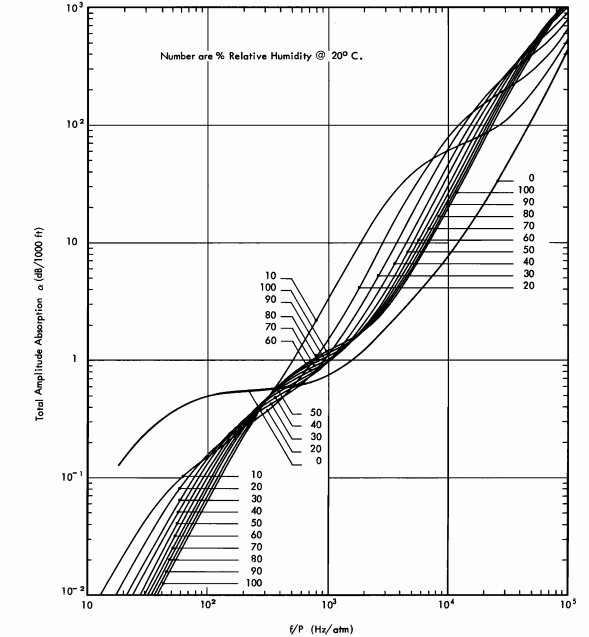
\includegraphics[width=0.8\textwidth]{Figures/airAbsorption.png}
\caption{Total absorption of sound in air as a function of frequency. The curves range from 0 to 100\% relative humidity and are for 20\degree C \cite{evans1972atmospheric} (Notice that the y-axis units are per 1000ft).}
\label{Fig:airAbsorption}
\end{figure}
\section{Atmospheric absorption} \label{app_atmabs}
Sound energy converts to heat as it travels through air. The conversion of sound-to-heat in air can happen due to conduction, shear viscosity or by molecular relaxation. The portion of sound absorbed by air becomes increasingly important as distance of propagation increases. For a plane wave, the loudness $L$ at a distance $x$ from a position of known loudness $L_0$ is given by
\begin{equation}
    L= L_0 - k.x,
\end{equation}
where k depends on the humidity, temperature, pressure as well as the molecular composition of atmosphere and is proportional to the square of the frequency. Thus, higher frequencies are absorbed by a far greater magnitude. This causes air to act as a low-pass filter over large distances. Molecular relaxation \cite{bass1990atmospheric}, \cite{evans1972atmospheric} is an important factor and losses due to oxygen-water vapour molecular relaxation are predominant above 500Hz. The absorption due to this factor is atleast 2 dB/kilometer irrespective of humidity and increases rapidly with frequency. The total absorption below 200 Hz is less than 1 dB/kilometer and decreases with frequency. If the air is extremely dry ($< 10\%$ relative humidity), the oxygen-carbon dioxide relaxation becomes significant and causes an almost constant absorption down from 500Hz to 80Hz of around 2dB/kilometer. The total air absorption as a function of frequency can be seen in Fig. \ref{Fig:airAbsorption}.

